\section{Overview}
\index{Overview}

What is a WebBrick? It is a network connected control and automation product designed around the principle 
of 'local control - global intelligence'. This means that most of the time control is handled locally but a 
system as a whole can be made more intelligent through the use of some central control
(for example the WebBrick Gateway) that provides the global intelligence. i.e. Lights for a room are a local issue, but heating is 
more of an overall control issue. This also means that you are
not dependant on a single control system for the complete system, you can always switch on the lights 
in this room while someone is making changes to a global control system.

Control can be done through a WebBrick's web interface, through its physical inputs or using remote commands.

\begin{figure}[H]
\centering
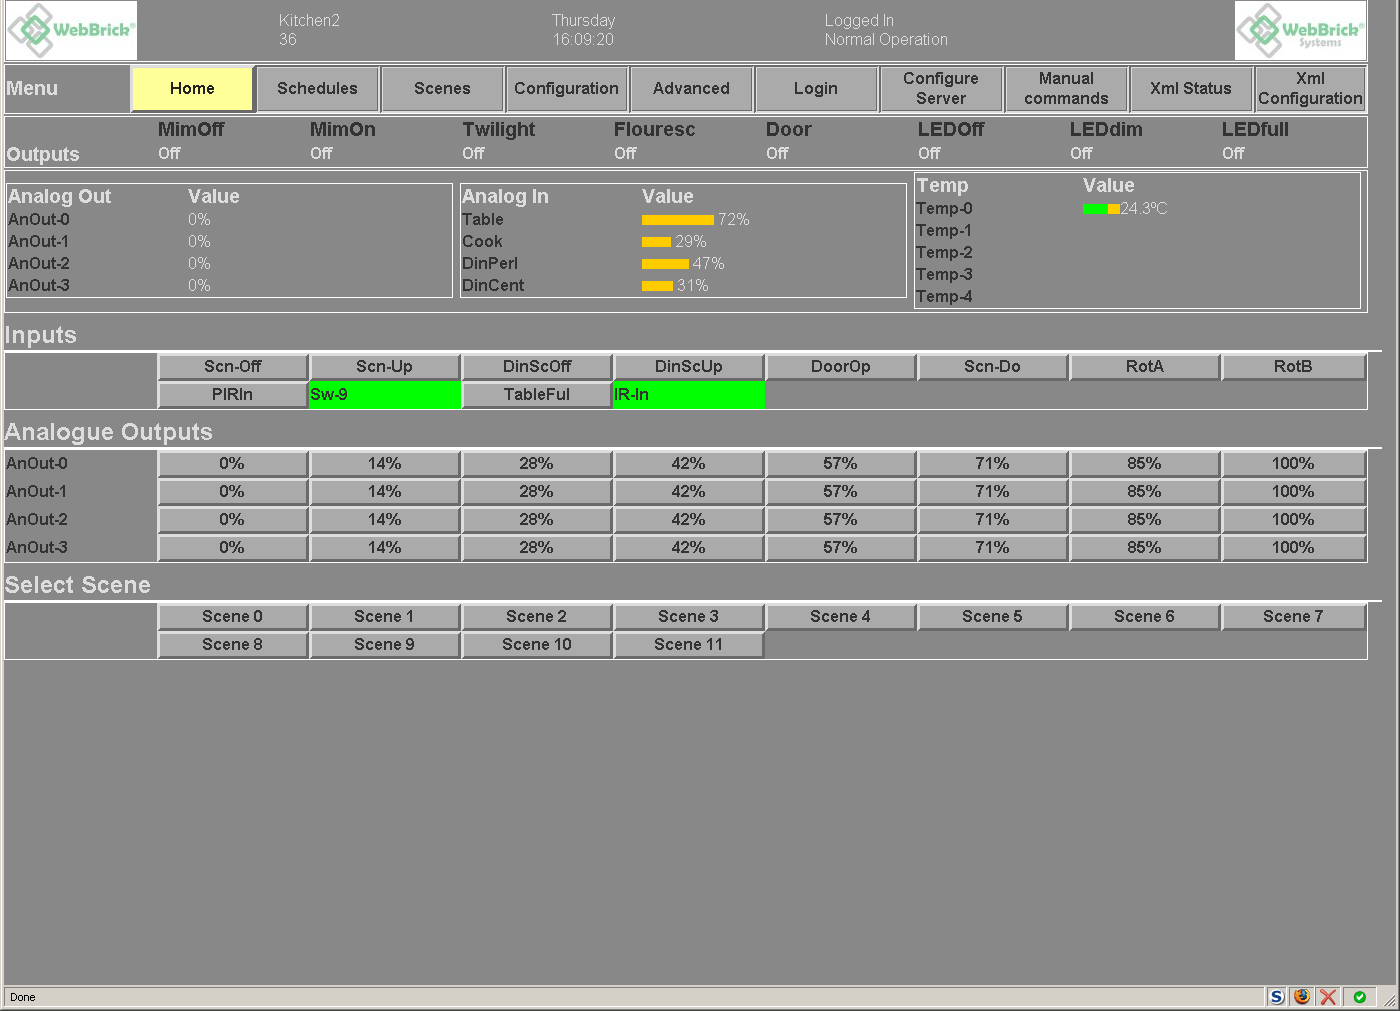
\includegraphics[width=0.9\textwidth]{Images/home.png}
\caption{Example of WebBrick Home Page}
\end{figure}
\subsection {History}

\index{History of WebBrick}

WebBrick started life as a bespoke project and in that incarnation there are 50-100 of them installed handling
tasks from building security to heating control, the largest setup uses 15+ WebBrick to manage a single house.
The latest incarnation (WebBrick6-64) is a commercial project with added facilities.
The V6 WebBrick has an added IO board which provides screw terminals for all connections. It also has 4 Mains switching 
triac�s and 2 Double pole changeover relays as well. We can also produce bespoke versions of the IO board
for specific uses.

\subsection {The Version 6.1 WebBrick}

The V6.1 WebBrick has the following connections:

\index{connections}

\begin{enumerate}
\item
8 Digital Outputs available as TTL and Open Collector drives, with an option for 8 more on bespoke developments. 
In the default configuration 4 of the digital outputs are connected to mains triac�s and can handle up to 500W 
per channel with a maximum of 1500W across all 4 channels. 2 Of the Open collector outputs are connected to double pole changeover relays.

\item
	8 Mimic outputs.  These are available at TTL level are are used to indicate the state of the Digital Outputs above.
	The main functions of these mimics is to drive indicator LEDs found on push buttons.

\item
8 Digital Trigger Inputs, TTL level - These can be treated as de-bounced push-buttons or toggle [MK] style inputs.  
	The actual trigger point can be the rising edge, falling edge or both.   
\item
4 Digital Inputs, As above but with no internal pull-up resistors [These were 'Monitors' on the series 6.0 WebBricks].
\item
4 Analogue Outputs 0-10V
\item
1 Rotary Encoder connection, currently used to adjust Analogue output 1. (To be extended to 4).
\item
4 Analogue Inputs This is a 0-5V input, high impedance, care must be taken not to exceed 5V on this pin, 
the web interface displays 0-100.
\item
One Wire Bus for up to 5 off Dallas DS18B20 temperature sensors.
\item
RJ45 connection for 10Mb/s Ethernet
\item
12V power connection
\end{enumerate}

\subsection {The Hardware}
A WebBrick is a PIC processor chip connected to a Netmedia SitePlayer Web CoProcessor, the later
provides the web interface and general IP networking connectivity.

\subsection {The Software}

The WebBrick is programmed in C and the siteplayer/User interface in html and Javascript. To provide
global intelligence a gateway system coordinates a network of WebBrick�s, this uses a combination of Apache,
PHP and Python. API libraries are provided for third party enhancements.

